\section{Pianificazione}
La pianificazione del lavoro all'interno del gruppo \textit{Zeus Code} segue i canoni dettati nella sezione \hyperlink{scadenze}{sottosezione 1.5}, la pianificazione di progetto viene suddivisa nelle seguenti fasi:
\begin{enumerate}
	\item \textbf{Analisi};
	\item \textbf{Consolidamento dei requisiti};
	\item \textbf{Progettazione architetturale};
	\item \textbf{Progettazione di dettaglio e codifica};
	\item \textbf{Validazione e collaudo}.
\end{enumerate}
Ogni fase consiste in un insieme di attività aventi una data di inizio e una di fine, il tutto viene riportato nei diagrammi di Gantt\glo. Viene fissata come data di scadenza il giorno di consegna dei materiali prodotti dalle attività. 
\subsection{Analisi}
\textit{Periodo: dal 2019-01-03 al 2019-04-19}\\
L'inizio di questa fase coincide con la formazione dei gruppi del secondo lotto e la fine corrisponde con la data ultima per la consegna dei documenti relativi alla revisione dei requisiti.
Questa fase è stata scomposta nelle seguenti sotto attività:
\begin{itemize}
	\item \textbf{Individuazione degli strumenti}: vengono scelti gli strumenti che saranno impiegati per la parte riguardante le comunicazioni tra membri, vengono inoltre definiti i programmi utili alla scrittura di file \LaTeX; 
	\item \textbf{Norme di Progetto}: utilizzando gli strumenti sopra indicati si stende il documento \textit{Norme di progetto v1.0.0} indipendente dal capitolato scelto. Il documento Norme di Progetto viene redatto dall'\textit{Amministratore} per conto del \textit{Responsabile di progetto};
	\item \textbf{Studio di fattibilità}: è compito degli \textit{Analisti} effettuare uno studio dei vari capitolati per evidenziarne pregi e difetti e scegliere il capitolato da sviluppare. Fase bloccante per l'Analisi dei Requisiti;
	\item \textbf{Analisi dei Requisiti}: questa attività è volta alla produzione del documento \textit{Analisi dei requisiti v1.0.0}, questo file è in continua fase di miglioramento fino alla data di consegna;
	\item \textbf{Piano di Progetto}: il \textit{Responsabile} analizza le singole attività e le loro date di scadenza in modo da gestire le risorse necessarie al loro completamento, viene redatto il documento \textit{Piano di progetto v1.0.0};
	\item \textbf{Piano di Qualifica}: attività volta alla redazione del file \textit{Piano di qualifica v1.0.0}, il quale individua le metodologie implicate nel garantire la qualità del prodotto; 
	\item \textbf{Glossario}: documento volto a racchiudere tutti termini che possono risultare ambigui o che semplicemente necessitano di una descrizione appropriata onde evitare incomprensioni.
\end{itemize}
%DA METTERE GANTT
%\begin{figure}[H]
%	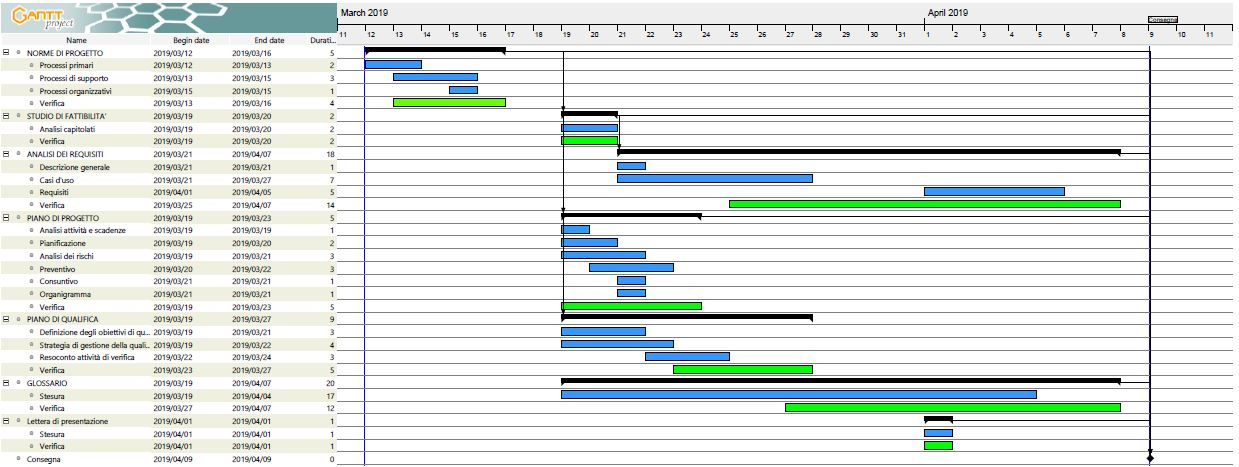
\includegraphics[width=0.99\linewidth]{res/images/gantt_analisi.jpg}
%	\caption{Diagramma di Gantt della fase di Analisi}
%\end{figure}

\subsection{Consolidamento dei requisiti}
\textit{Periodo: dal 2019-03-28 al 2019-04-19} \\
Questa fase ha inizio dopo l'attività di analisi e termina con la consegna dei documenti per la revisione dei requisiti. Le attività 
di questa fase sono:
\begin{itemize}
	\item \textbf{Consolidamento}: vengono migliorati i requisiti ottenuti nella fase di analisi;
	\item \textbf{Preparazione alla presentazione}: viene pianificata la scaletta da seguire per la presentazione del 2019-04-19;
	\item \textbf{Incremento e Verifica}: vengono rivalutati singolarmente tutti i file e in caso saranno soggetti a miglioramenti e modifiche;
	\item \textbf{Approfondimento personale}: i membri del team dedicheranno un monte ore, da loro predisposto, per studiare le nuove tecnologie richieste dal capitolato\glo.Questa attività verrà svolta in modo autonomo e quindi non è riportata nel seguente diagramma di Gantt~\ref{fig:gantt_con}.
\end{itemize}
%
%\begin{figure}[H]
%	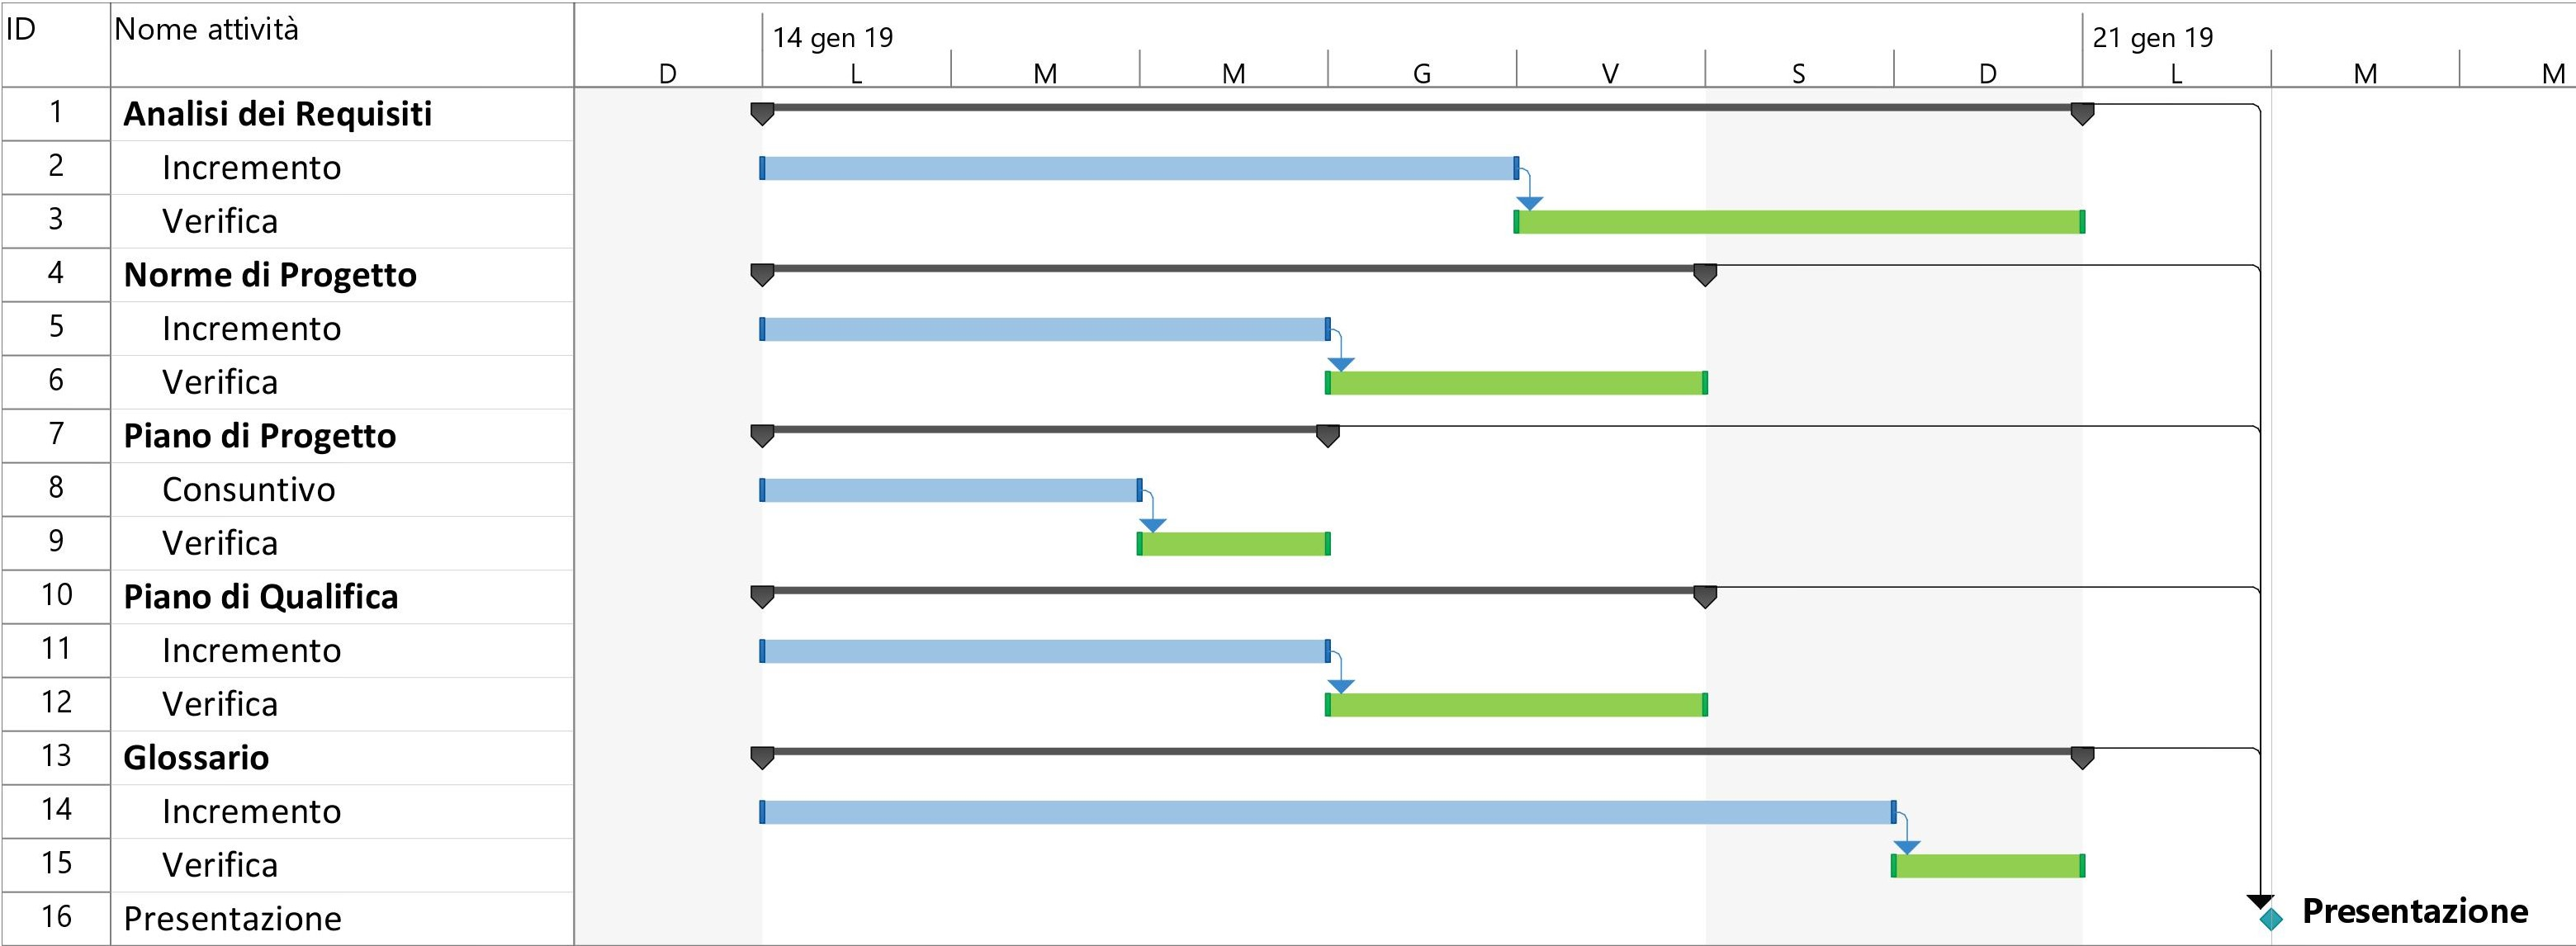
\includegraphics[width=0.99\linewidth]{res/images/gantt_cons.jpg}
%	\caption{Diagramma di Gantt della fase di Consolidamento dei requisiti}
%	\label{fig:gantt_con}
%\end{figure}

%-----------------Sottosezione Progettazione Architetturale---------------------
\subsection{Progettazione architetturale}
\textit{Periodo: dal 2019-04-19 al 2019-03-08} \\
Questa fase comincia il giorno successivo alla presentazione e la fine coincide con la data di consegna Revisione di 
Progettazione. In questo periodo verrà individuata una soluzione architetturale 
tale per cui i requisiti richiesti vengano soddisfatti.
\begin{itemize}
	\item \textbf{Technology Baseline}: viene redatto l'
	Allegato Tecnico  nel quale vengono 
	individuati i design 
	pattern\glosp che verranno adottati per lo sviluppo. Inoltre il documento 
	include il tracciamento dei requisiti.\\
	Infine viene codificato il \textbf{Proof of Concept}\glosp il 
	quale viene presentato o condiviso tramite repository al committente e 
	proponente in una data da definirsi;
	\item \textbf{Incremento e Verifica}: se necessario vengono migliorati i 
	documenti prodotti nelle fasi precedenti.
\end{itemize}

\begin{figure}[H]
	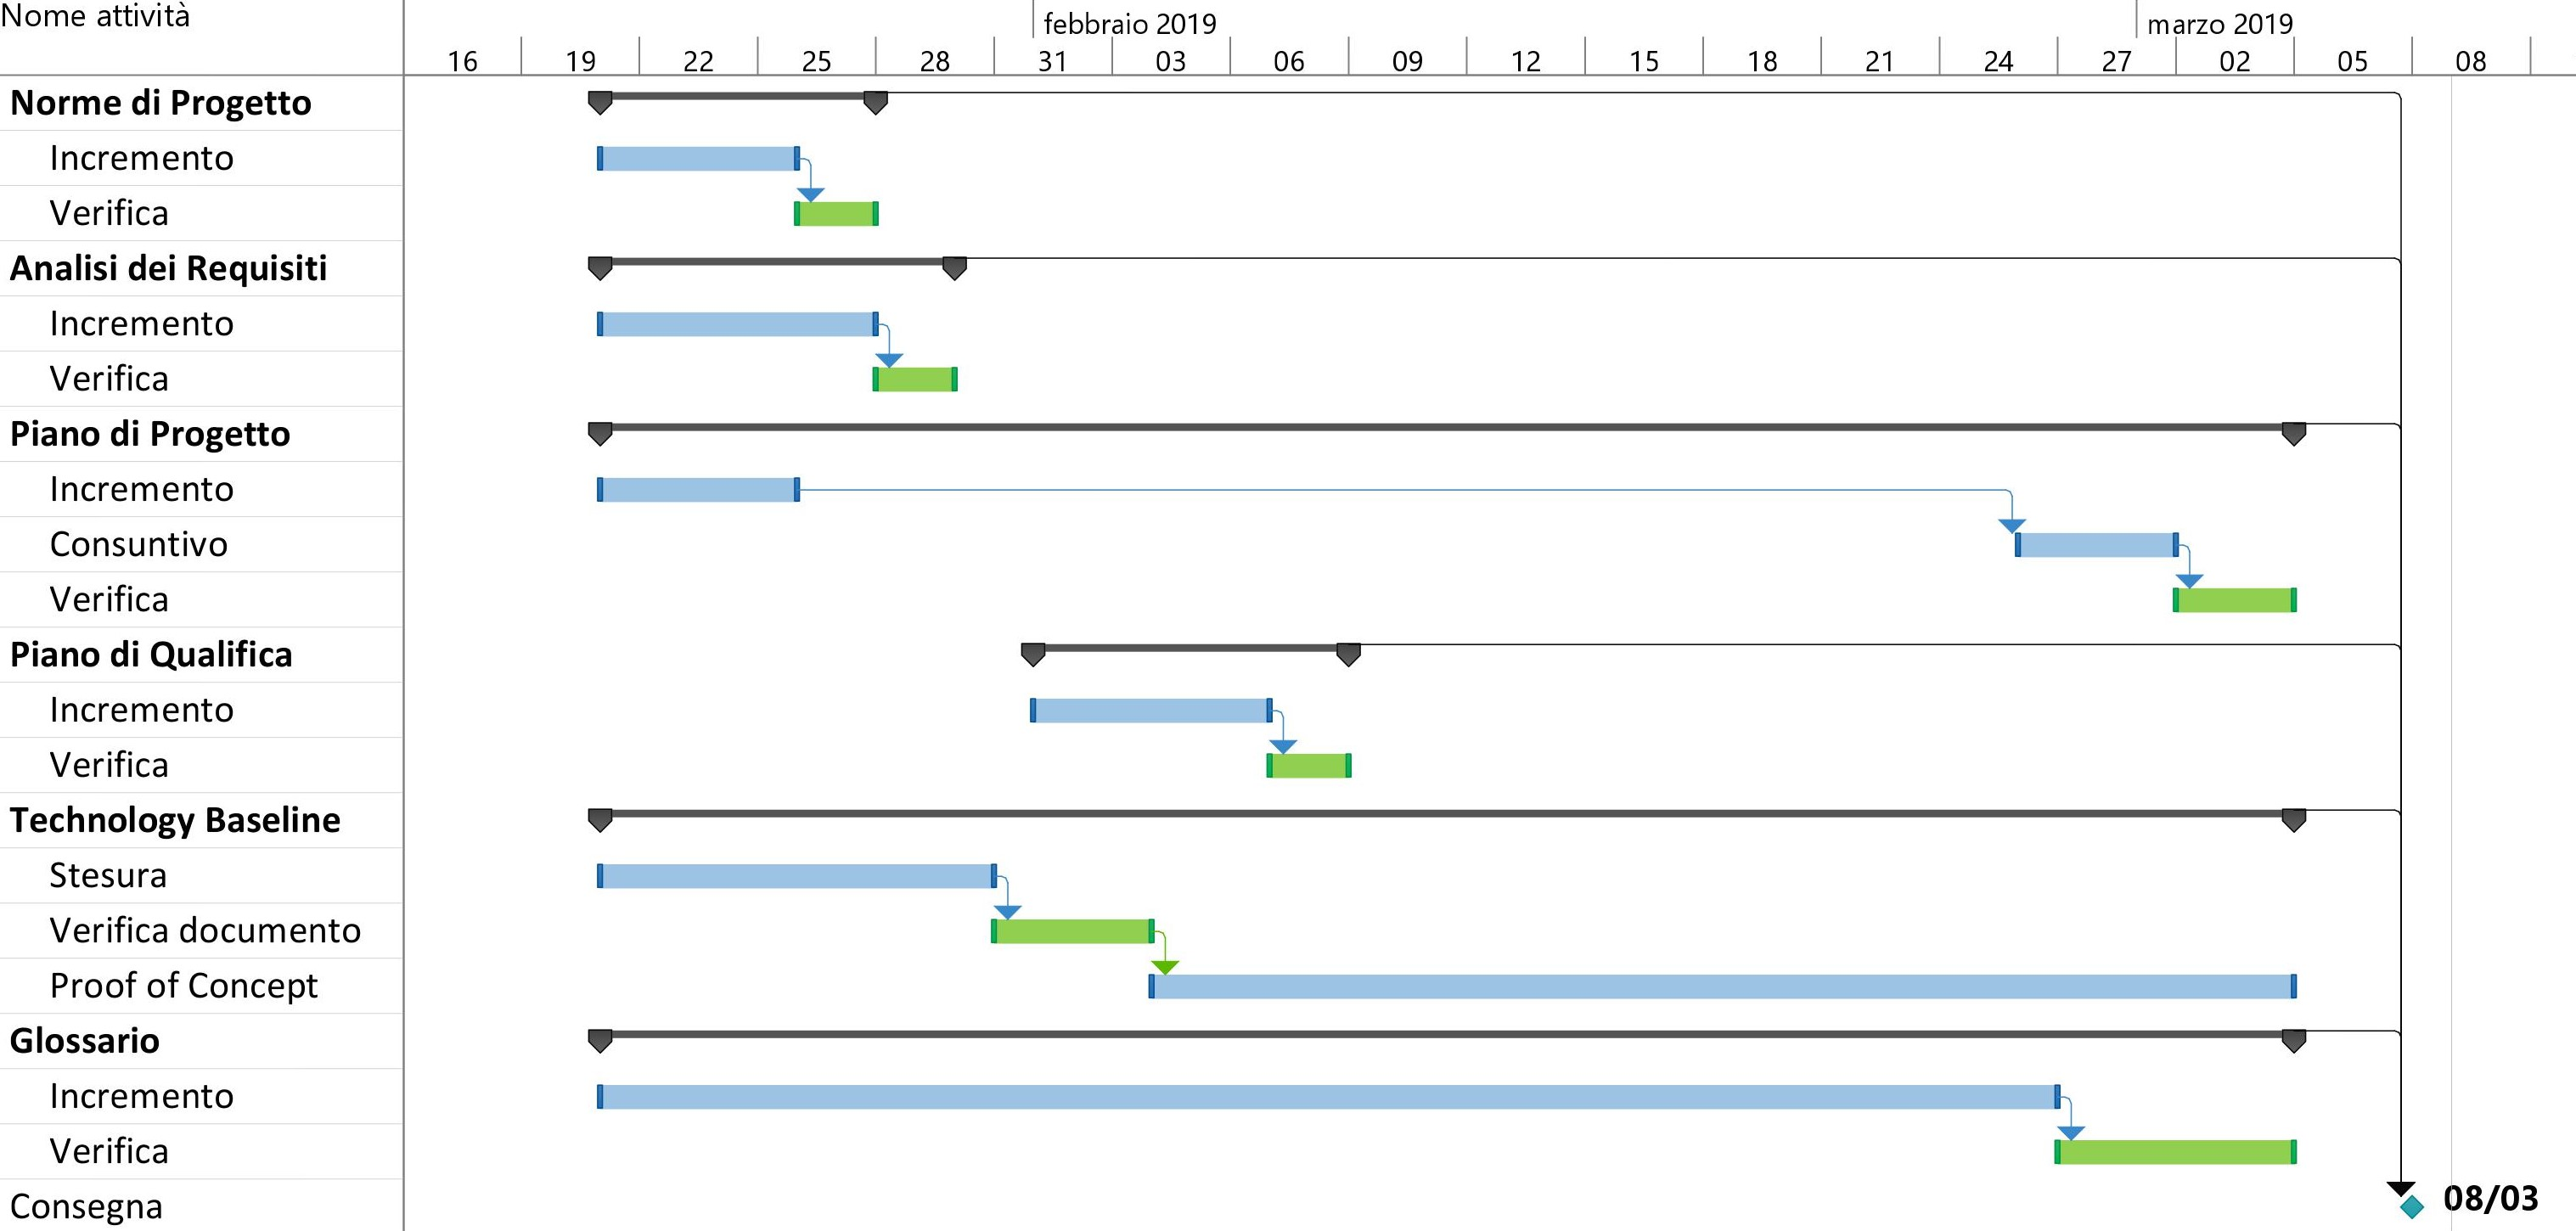
\includegraphics[width=0.99\linewidth]{res/images/gantt_pa.jpg}
	\caption{Diagramma di Gantt della fase di Progettazione architetturale}
\end{figure}


%-------------------Sottosezione Progettazione di Dettaglio---------------------
\subsection{Progettazione di dettaglio e codifica}
\textit{Periodo: dal 2019-03-15 al 2019-04-12}
L'inizio di questa fase è il giorno della scadenza della \textit{Revisione di 
Progettazione} e la data di fine coincide con la data di consegna dei documenti 
in vista della \textit{Revisione di Qualifica}. Le attività di questa fase sono:
\begin{itemize}
	\item \textbf{Product Baseline}: a seguito della \textit{Technology 
	Baseline} l'architettura individuata in essa viene scomposta nelle sue unità,
	che sono analizzate in profondità per fornire i 
	dettagli necessari alla loro codifica e verifica. A supporto 
	di ciò viene redatto l'Allegato Tecnico di supporto alla Product Baseline;
	\item \textbf{Codifica}: questa attività consiste nella scrittura del 
	codice e della sua verifica con modalità e strumenti definiti nel 
	\textit{Piano di Qualifica v2.0.0}
	\item \textbf{Manuale Utente}: viene redatto il documento \textit{Manuale 
	Utente} atto a fornire istruzioni e indicazioni per l'utilizzo del prodotto;
	\item \textbf{Incremento e Verifica}: se necessario vengono migliorati i 
	documenti prodotti nelle fasi precedenti.
\end{itemize}

\begin{figure}[H]
	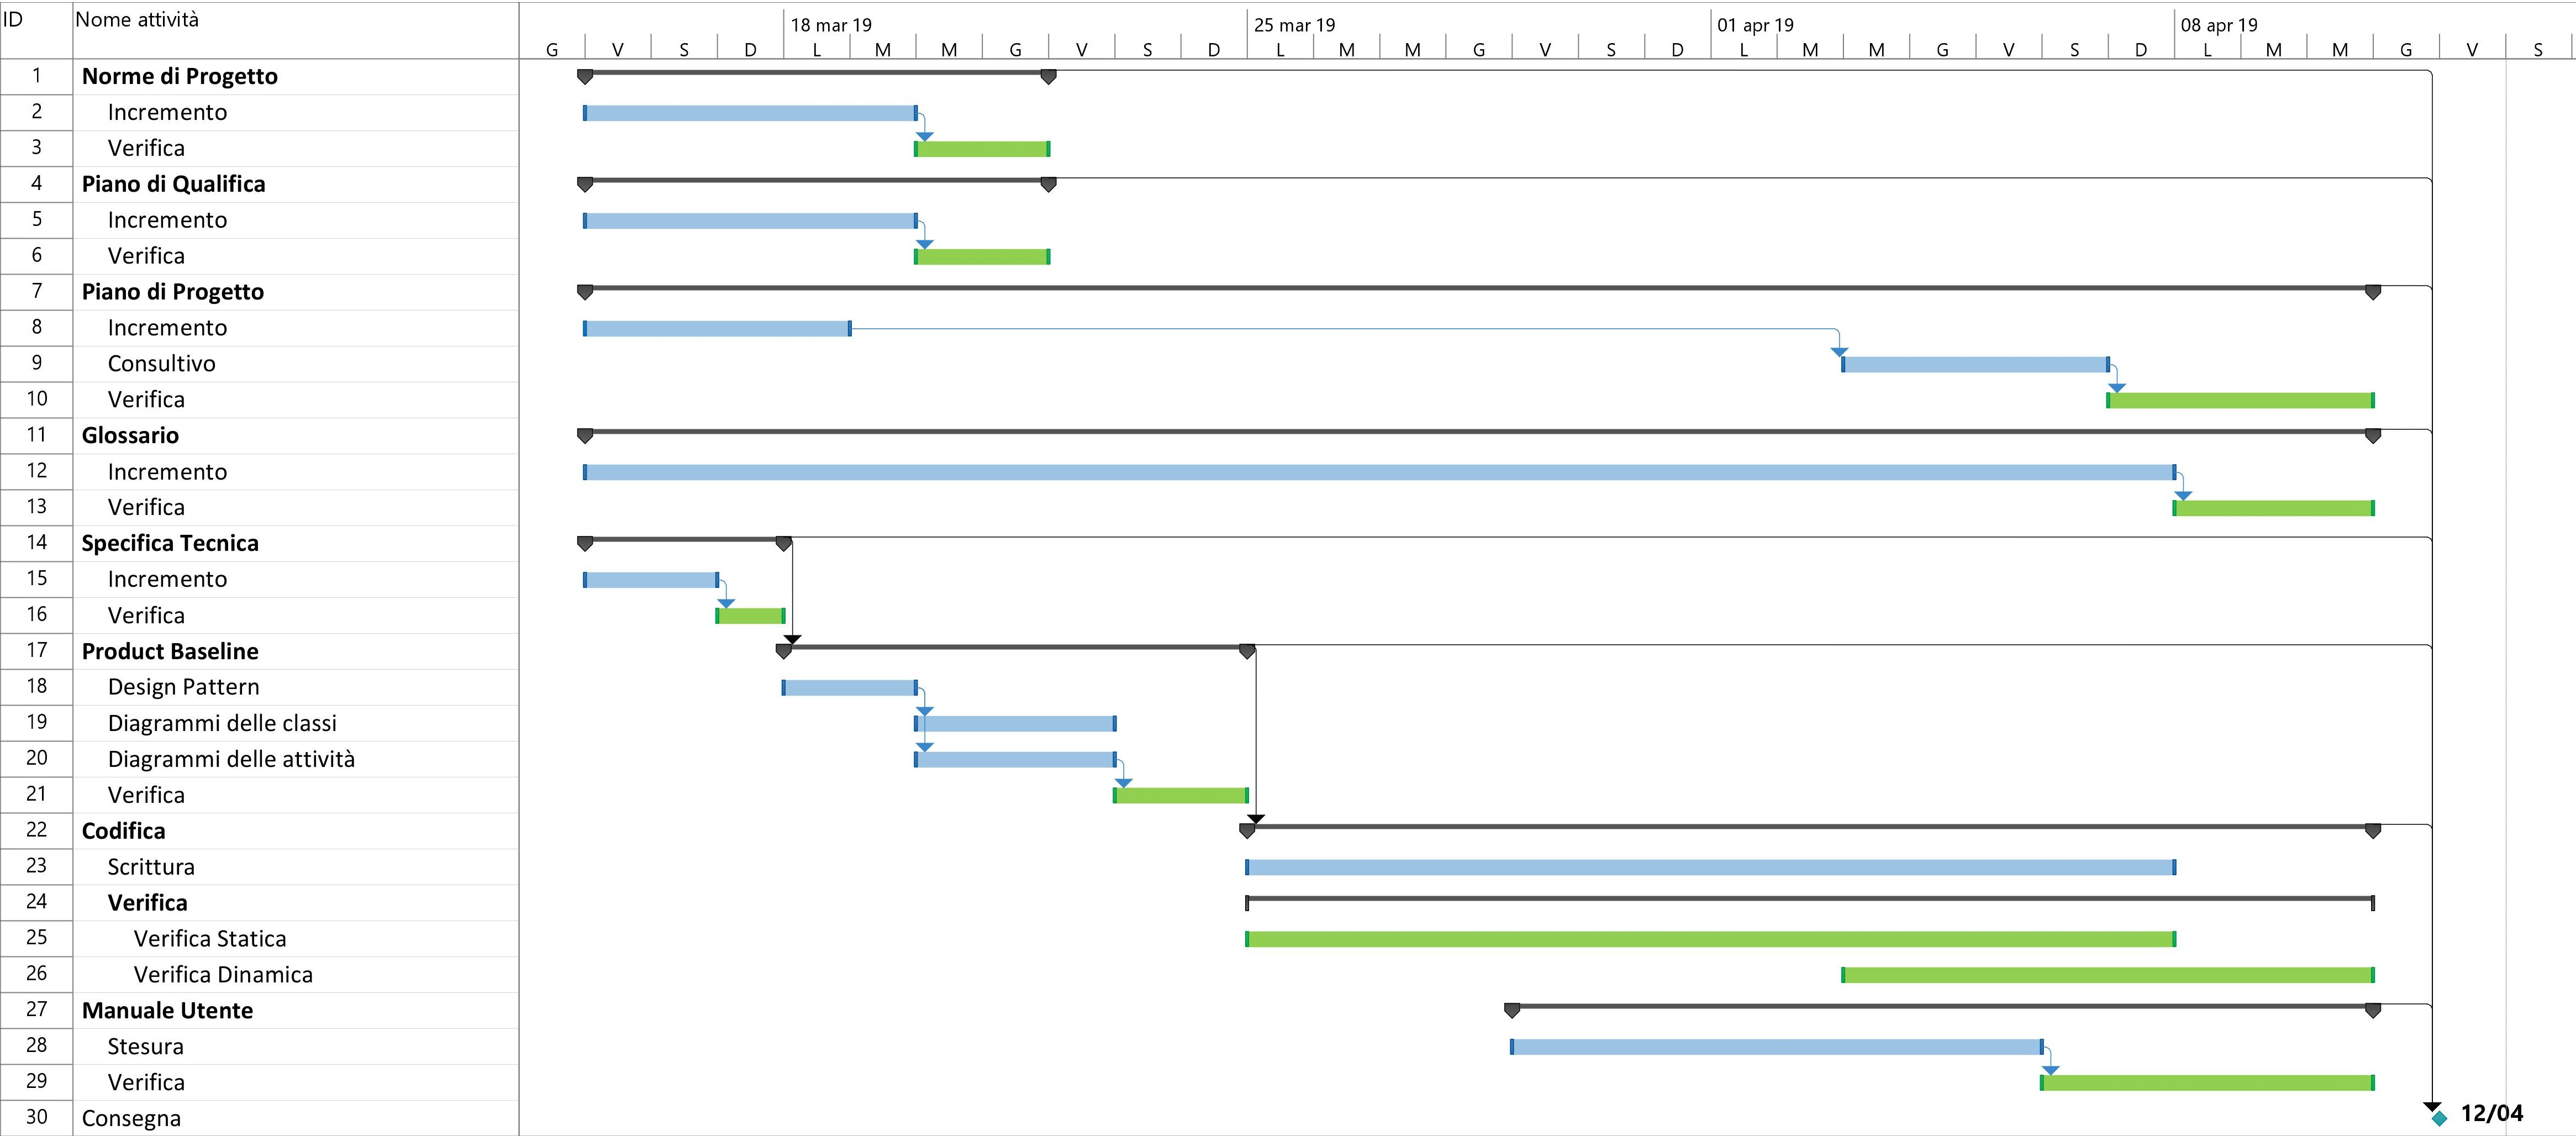
\includegraphics[width=0.99\linewidth]{res/images/gantt_pd.jpg}
	\caption{Diagramma di Gantt della fase di Progettazione di dettaglio e codifica}
\end{figure}
\pagebreak


\subsection{Validazione e collaudo}
\textit{Periodo: dal 2019-04-12 al 2019-05-17 } \\
L'inizio di questa fase coincide con la data di consegna dei documenti per la 
\textit{Revisione di Qualifica}, mentre la data di fine coincide con la 
consegna in vista della \textit{Revisione di Accettazione}. Durante questo periodo 
si eseguiranno ulteriori attività di validazione e verifica. Le attività 
previste sono: 
\begin{itemize}
	\item \textbf{Validazione e Collaudo}: per la parte di collaudo si 
	eseguiranno ulteriori test sul prodotto, in modo da garantirne la 
	correttezza e stabilità. Per la parte di validazione, verrà 
	valutata la coerenza del prodotto e dei requisiti specificati nel documento 
	\textit{Analisi dei Requisiti} nella sua ultima versione;
	\item \textbf{Manuale Sviluppatore}: viene redatto il documento \textit{Manuale Sviluppatore} atto a fornire tutte le informazioni necessarie al mantenimento, manutenzione e ampliamento del prodotto finale;
	\item \textbf{Incremento e Verifica}: se necessario vengono migliorati i 
	documenti prodotti nelle fasi precedenti.
\end{itemize}
\begin{figure}[H]
	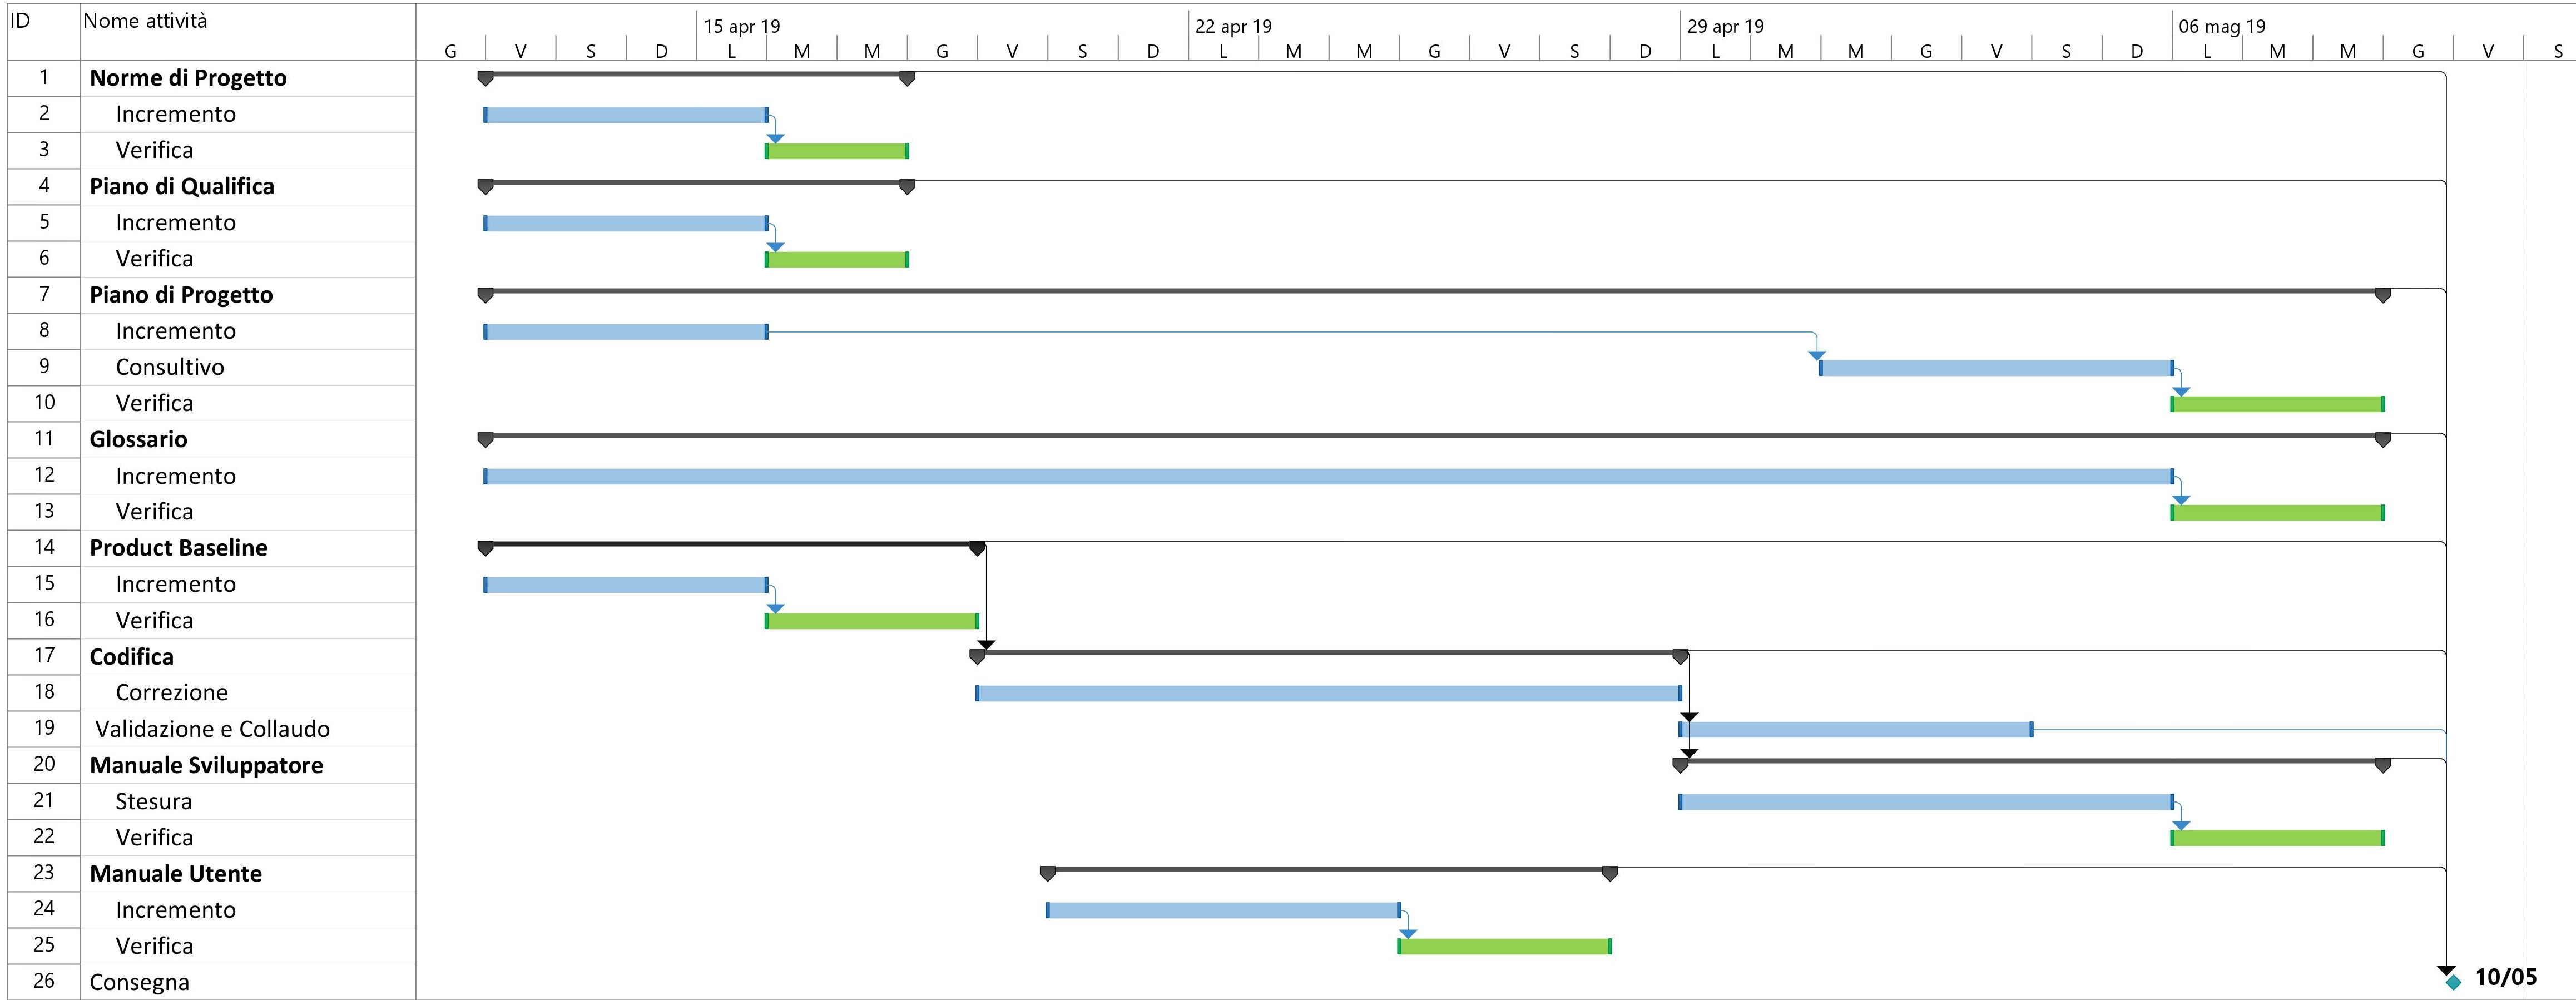
\includegraphics[width=0.99\linewidth]{res/images/gantt_val.jpg}
	\caption{Diagramma di Gantt della fase di Validazione e collaudo}
\end{figure}